% ---- ETD Document Class and Useful Packages ---- %
\documentclass{ucetd}
\usepackage{subfigure,epsfig,amsfonts}
\usepackage{natbib}
\usepackage{amsmath}
\usepackage{amssymb}
\usepackage{amsthm}
\usepackage[toc,page]{appendix}
\usepackage[labelfont=bf]{caption}
\usepackage{rotating}
\usepackage[dvipsnames]{xcolor}
\usepackage{url}
\usepackage{bm}
\usepackage{bbm}
\usepackage{comment}

%% Use these commands to set biographic information for the title page:
\title{Visualizing nucleosome phase separation with super resolution microscopy}
\author{Clayton W. Seitz}
\department{Department of Physics}
\division{Preliminary Examination}
\degree{PhD Preliminary Examination}
\date{Fall 2023}

%% Use these commands to set a dedication and epigraph text

\epigraph{Epigraph}



\begin{document}
%% Basic setup commands
% If you don't want a title page comment out the next line and uncomment the line after it:
\maketitle
%\omittitle

% These lines can be commented out to disable the copyright/dedication/epigraph pages
%\makecopyright
%\makededication


%% Make the various tables of contents
\tableofcontents
%\listoftables

%\acknowledgments
% Enter Acknowledgements here

\abstract

Single-molecule localization microscopy (SMLM) techniques, such as direct stochastic optical reconstruction microscopy (dSTORM), can be used to produce a pointillist representation of nucleosome organization at diffraction-unlimited precision. Direct STORM approaches leverage the deactivation of standard fluorescent tags, followed by spontaneous or photoinduced reactivation, which can be used to achieve super-resolution reconstructions of nuclear proteins and nucleic acids. This basic principle remains one of the method's primary limitations - standard SMLM fitting routines require tight control of activation and reactivation to maintain sparse emitters, presenting a tradeoff between imaging speed and labeling density. Here, I present two parallel projects, which are closely related, but separable. The first represents a novel technique for dense stochastic optical reconstruction microscopy based on deep learning and photon statistics. In the second, conventional dSTORM is adapted for live cell imaging of chromatin nanodomains and physical analysis of their associations with BRD4 - a well known component of phase separated condensates in mammalian nuclei. 

\clearpage

\mainmatter



\section{Introduction}

\subsection{Single molecule localization microscopy}

Single molecule localization microscopy (SMLM) relies on the temporal resolution of fluorophores in the sample whose spatially overlapping point spread functions would otherwise render them unresolvable at the detector. SMLM techniques, such as stochastic optical reconstruction microsscopy (STORM) and photo-activated localization microscopy (PALM) remain desirable for super-resolution imaging of many cellular structures, due to their cost-effective implementation and diffraction unlimited resolution (Schermelleh 2019). Common strategies for the temporal separation of molecules involve transient intramolecular rearrangements to switch from dark to fluorescent states or the exploitation of non-emitting molecular radicals. For direct STORM, rhodamine derivatives can undergo intersystem crossing to a triplet state, which can be reduced by thiols to form a dark radical species. The dark state can then be quenched by oxidative processes, driving the fluorophore back to its ground state (Figure 1). Long dark state lifetimes are commonly used in STORM imaging, while quenching results in higher duty cycle photoswitching and increased rates of photobleaching due to irreversible oxidative damage of important functional groups.

The spatial resolution of SMLM images can be directly computed from the variance of a statistical estimator of molecular coordinates, using the Fourier ring correlation (Nieuwenhuizen 2013). This variance is an aleatoric or systematic uncertainty, often of a maximum likelihood estimator, and is bounded from below by the inverse of the Fisher information matrix, known as the Cramer-Rao lower bound (Chao 2016). Localization uncertainties are commonly tens of nanometers, although recent work on integration of Bayesian priors with modulation enhanced single molecule localization microscopy (meSMLM) has reduced spatial resolution below 1 nanometer (Kalisvaart 2022). Nevertheless, fluorescent labeling density still remains a major bottleneck to SMLM acqusitions. Static uncertainty due to molecular crowding can be partially amelioriated by using pairwise or higher-order temporal correlations within a pixel neighborhood, known as stochastic optical fluctuation imaging or SOFI (Dertinger 2009). Other approaches such as stimulated emission and depletion (STED) imaging bring control over the photophysical state of a chosen subset of the sample, yet the need for laser scanning prevents widespread application in live-cell studies. At the same time, the spatial resolution and relative simplicity of SMLM techniques remains unmatched, inciting an effort to increase the resolution of SMLM techniques and explore avenues towards time resolved SMLM.

\begin{figure}
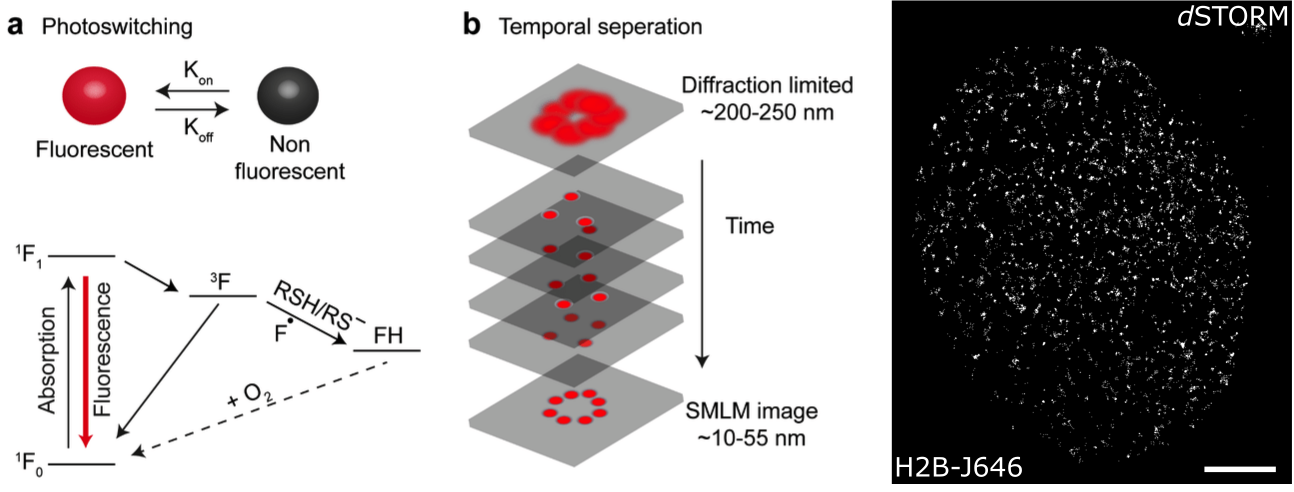
\includegraphics[width=\textwidth]{Intro.png}
\caption{\textbf{Stochastic optical reconstruction microscopy (STORM)}. (A) Single molecules are resolved by separating their fluorescent emission in time, using fluorophores with multiple photophysical states (B) Example super-resolution image of H2B protein in a living Hela cell nucleus and the first frame of a STORM time series (inset). (C) Photophysics of tetramethylrhodamine (TMR) and its derivatives JF549 and JF646. Maximum absorption occurs at 549nm or 646nm respectively and return to the ground state can occur via twisted internal charge transfer or inter-system crossing (Grimm 2021)}
\end{figure}


\begin{figure}
\begin{center}
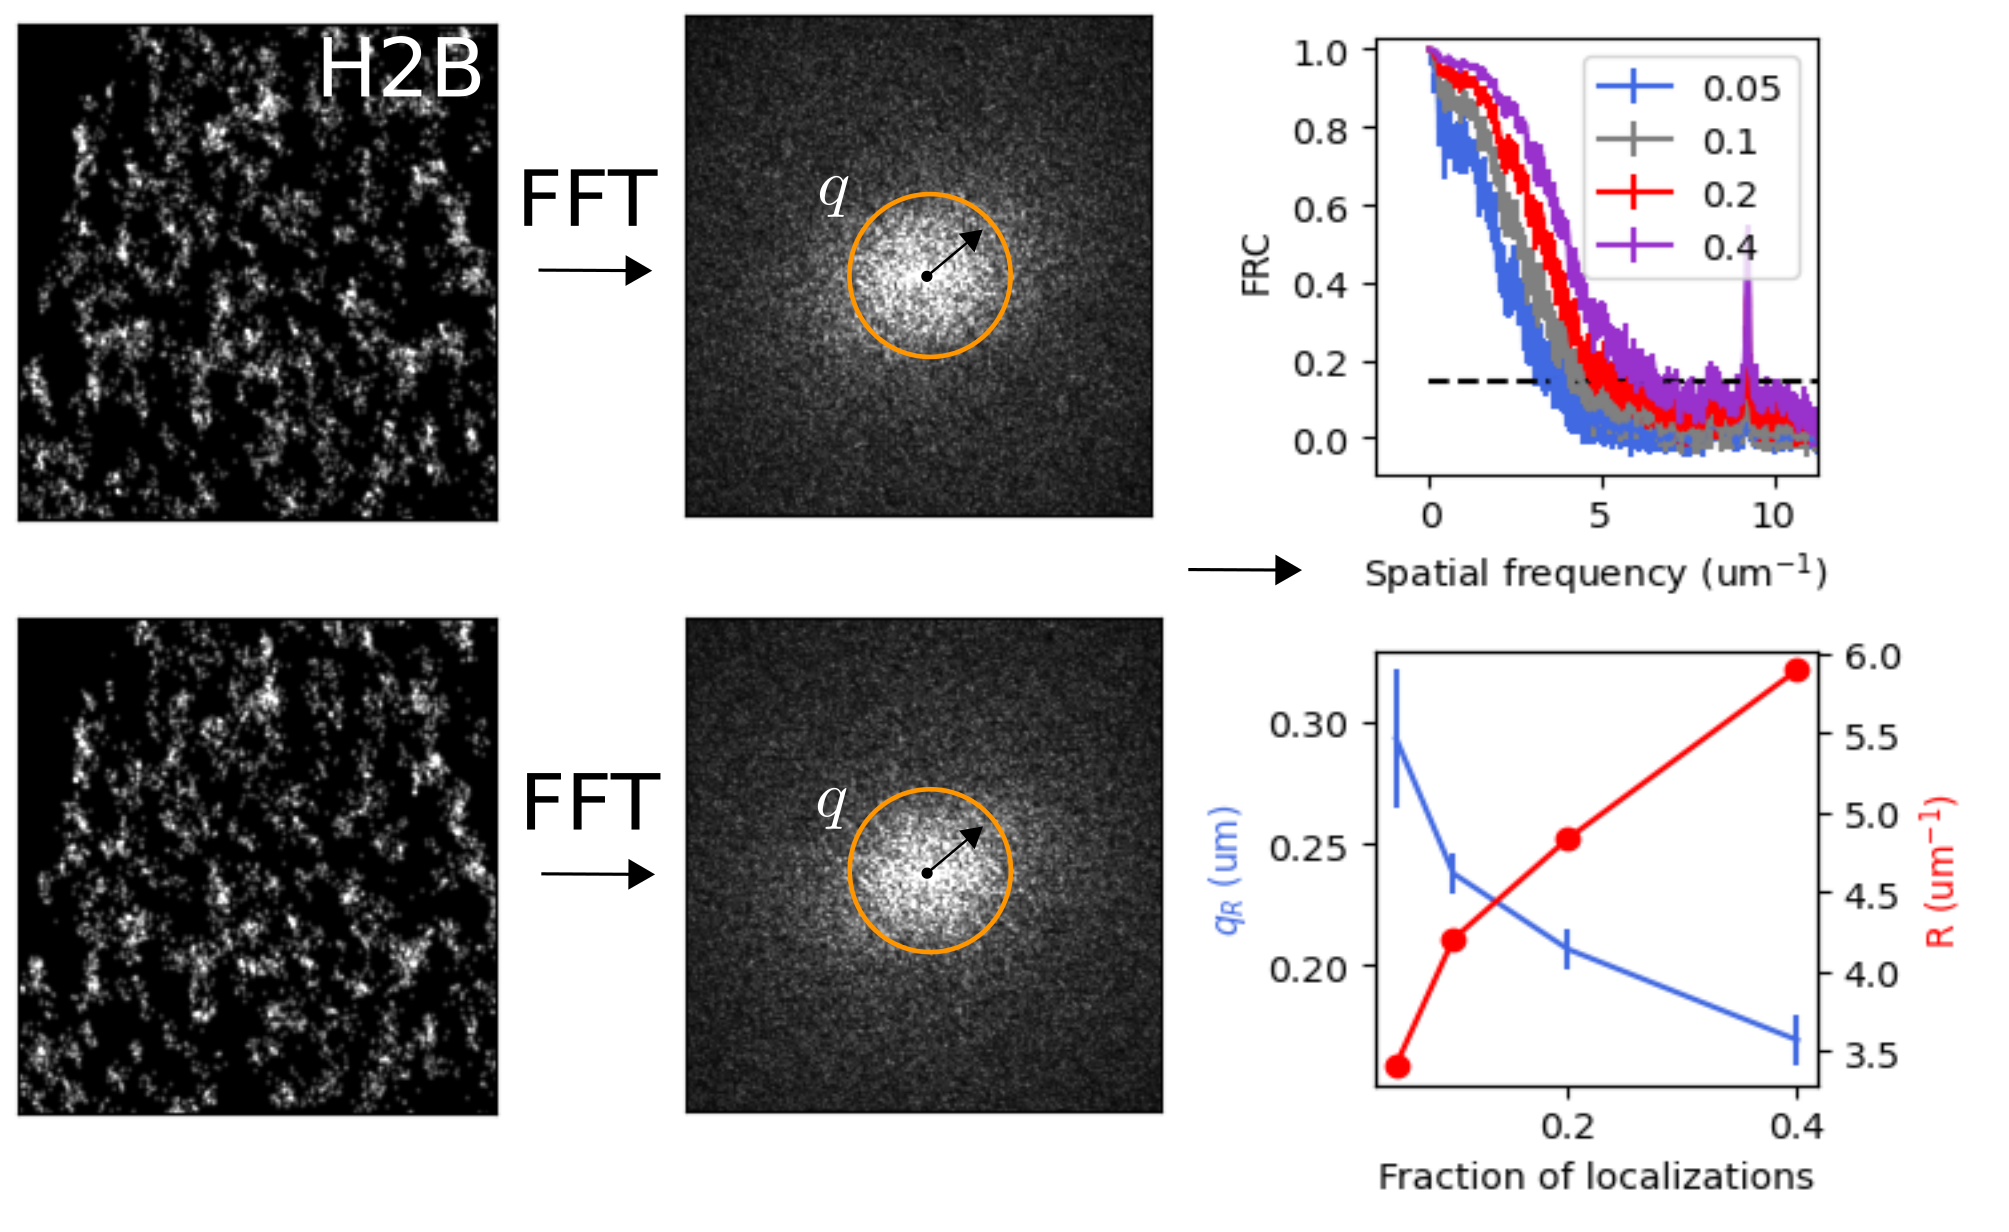
\includegraphics[width=13cm]{FRC.png}
\end{center}
\caption{\textbf{Dense localization increases image resolution and enables time-resolved STORM}. A pair of subsets is drawn from the full list of localizations, and isotropic Gaussian kernel density estimation is performed. The Fourier Ring Correlation is calculated for the pair and plotted as a function of spatial frequency.}
\end{figure}


\subsection{Towards time-resolved SMLM}

Previous approaches to improving the resolution of SMLM have been primarily based on a combination of intensity measurements and probabilistic deep learning. In one approach, deep generative models have been used to learn the generating distribution of images of cellular structures from super-resolution data. Trained models can then be used to predict super-resolution images based on sparse localizations or widefield images (Ouyang 2018; Barth 2020; Chen 2023). Other approaches leverage convolutional neural networks to transform dense images into a localization map (Nehme 2020; Speiser 2021). Convolutional neural networks are well-known for their ability to use higher order spatial structure in an image to infer latent variables. In essence, this can be seen as learning a translation from SMLM image intensities to pixel-wise probabilities of emitter occupancy. Here, we enhance this second approach by going beyond standard intensity measurments, constraining localizations by counting fluorescent emitters with photon statistics.

Within the broader domain of super-resolution imaging, innovations in single photon detection technologies have begun to be integrated into fluorescence microscopes (Forbes 2019). Single photon detectors such as single photon avalanche photodiodes (SPADs) have orders of magnitude higher temporal resolutions than standard sCMOS cameras, single photon sensitivity, and theoretically zero readout noise. Such properties make these devices highly desirable for imaging applications; however, application of SPAD arrays in imaging have been limited to small bundles of a few tens of detector elements combined with laser scanning (Israel 2017; Forbes 2019; Tenne 2019). Recently, SPAD cameras have become commercially available, potentially bringing many of the advantages of single photon detection to widefield fluorescence microscopy. 

Isolated fluorescent emitters exhibit fluorescence antibunching, which means that fluorescence emission has sub-Poisson photon statistics. This property of fluorescence emission from a single emitter has been previously applied to counting fluorescent molecules in the spot of a confocal microscope (Ta 2010). Molecular counting with photon statistics has a fairly simple motivation: a photon emitted by a fluorescence molecule can only be detected once. Coincidence of photons at multiple detector elements provides evidence that two or more molecules are present in the imaged region. Using high speed cameras, we are able to directly model the total photon counts in a region of interest using a Hidden Markov Model (HMM). Under this formalism, the number of active fluorescent molecules in the ROI is modeled as a Markovian stochastic process, which is then measured according to the emission distribution of the HMM. Using model selection techniques, one can obtain estimates of the number of fluorescent emitters in the ROI by providing prior information about their emission statistics and scoring the observed sequence of counts. 

\subsection{Super-resolution of nucleosome-BRD4 interactions in living cells}

\begin{figure}
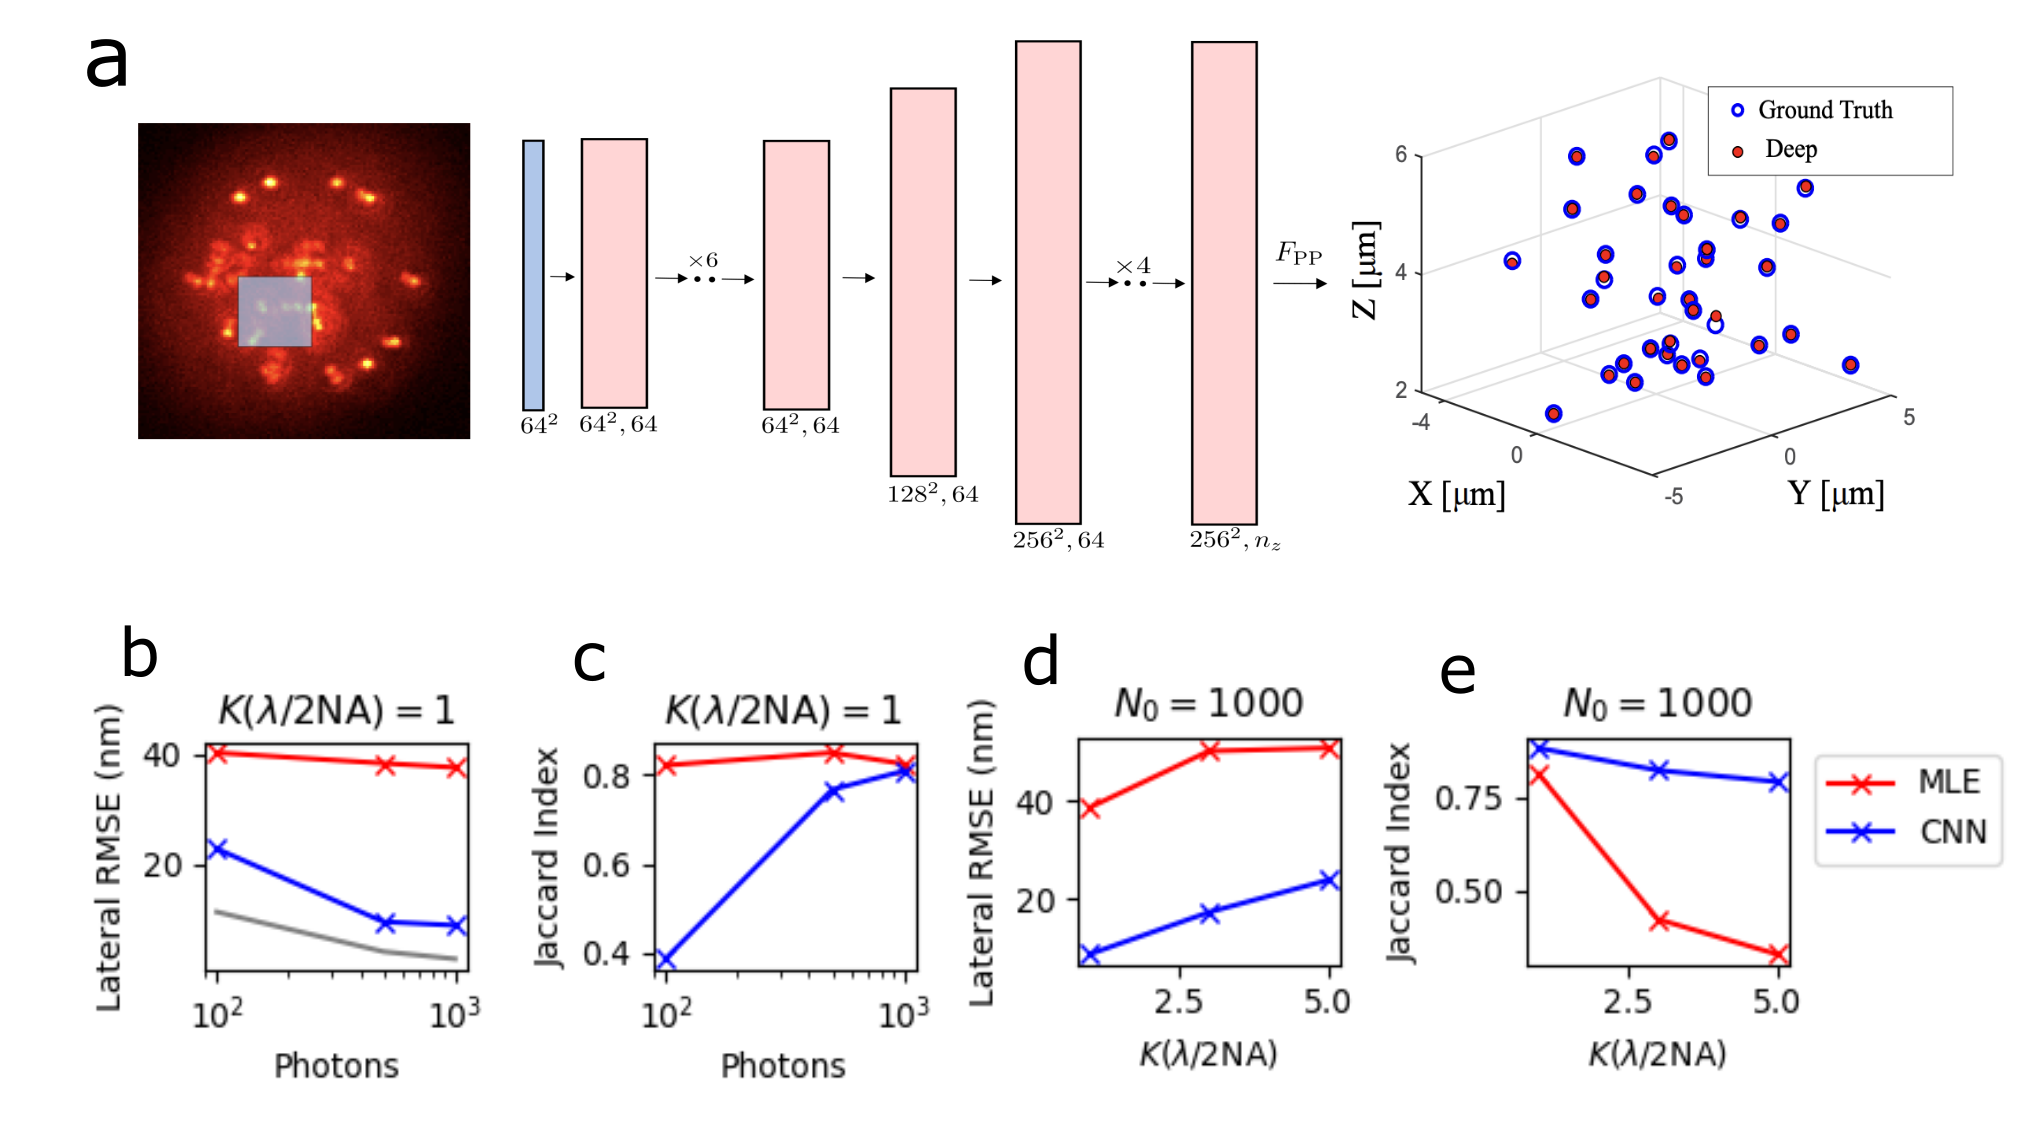
\includegraphics[width=\textwidth]{PSF2D.png}
\caption{\textbf{Deep networks outperform MLE in dense localization}} (A) DeepSTORM3D architecture with 612K trainable parameters used for localization. (B-E) Lateral root mean squared error of MLE and CNN estimators with respect to the incident photon count and the number of molecules within the diffraction limit $\lambda/2\mathrm{NA}$.
\end{figure}


Super-resolution imaging with intensity information alone remains a highly valuable technique, and we demonstrate this by live cell super-resolution imaging of nucleusome-BRD4 interactions in transcriptional condensates in the nucleus. The nucleosome is the fundamental unit of chromatin, which forms the basic scaffold for a variety of biomolecular processes in a cell nucleus. Super-resolved nucleosome organization has been studied extensively in various epigenomic states to reveal segregated nanoclusters, dispersed nanodomains, and compact large aggregates. Nucleosomes assemble into heterogeneous clusters of variable sizes, interspersed with nucleosome-depleted regions (Ricci 2015). Histones can be decorated with various post-translational modifications such as acetylation, methylation, phosphorylation, and ubiquination. The recruitment of proteins and complexes with specific enzymatic activities is now a well-accepted dogma of how modifications mediate their function. Histone modifications can influence transcription of genes, and many other DNA processes such as repair, replication and recombination (Bannister and Kouzarides, 2011). 

Here, study spatial nucleosome organization in living cells, with a particular focus on the structure of biomolecular condensates containing bromodomain protein 4 (BRD4) protein, a major tandem-bromodomain-containing transcriptional regulator. BRD4 plays an important role in diverse cellular functions such as transcription, replication, epigenetic regulation, and DNA repair, and has been implicated in cancer and autoimmune diseases. BRD4 acetylates Lysine 122 on H3 (H3K122), a residue critical for nucleosome stability, resulting in nucleosome eviction and chromatin decompaction (Devaiah 2016). The intrinsically disordered regions (IDRs) of BRD4 are thought to facilitate its phase separation with coactivators such as MED1. The phase separation properties of BRD4 have been well-studied in several cell lines (Han 2020), and in the context of super-enhancers (Sabari 2018).

Selective bromodomain inhibitors, such as JQ1 are often employed to displace BRD4 protein from chromatin (Filippakopoulos 2010). 1,6-hexanediol (1,6-HD), an aliphatic alcohol, can inhibit weak hydrophobic protein-protein interactions required for the droplet formation (droplet melting activity) and is widely used to elucidate the formation process of nuclear bodies (Duster 2021). However, the relationship of BRD4, and phase separation at large, with the spatial structure of nucleosome nanodomains remains unclear. As BRD4 is a critical component of phase separated transcriptional condensates, we envision a complementary approach, consisting of specific and non-specific inhibition of BRD4-containing condensates using small molecle drugs and BRD4 mutation or knockdown.


\section{Results}

\begin{figure}
\begin{center}
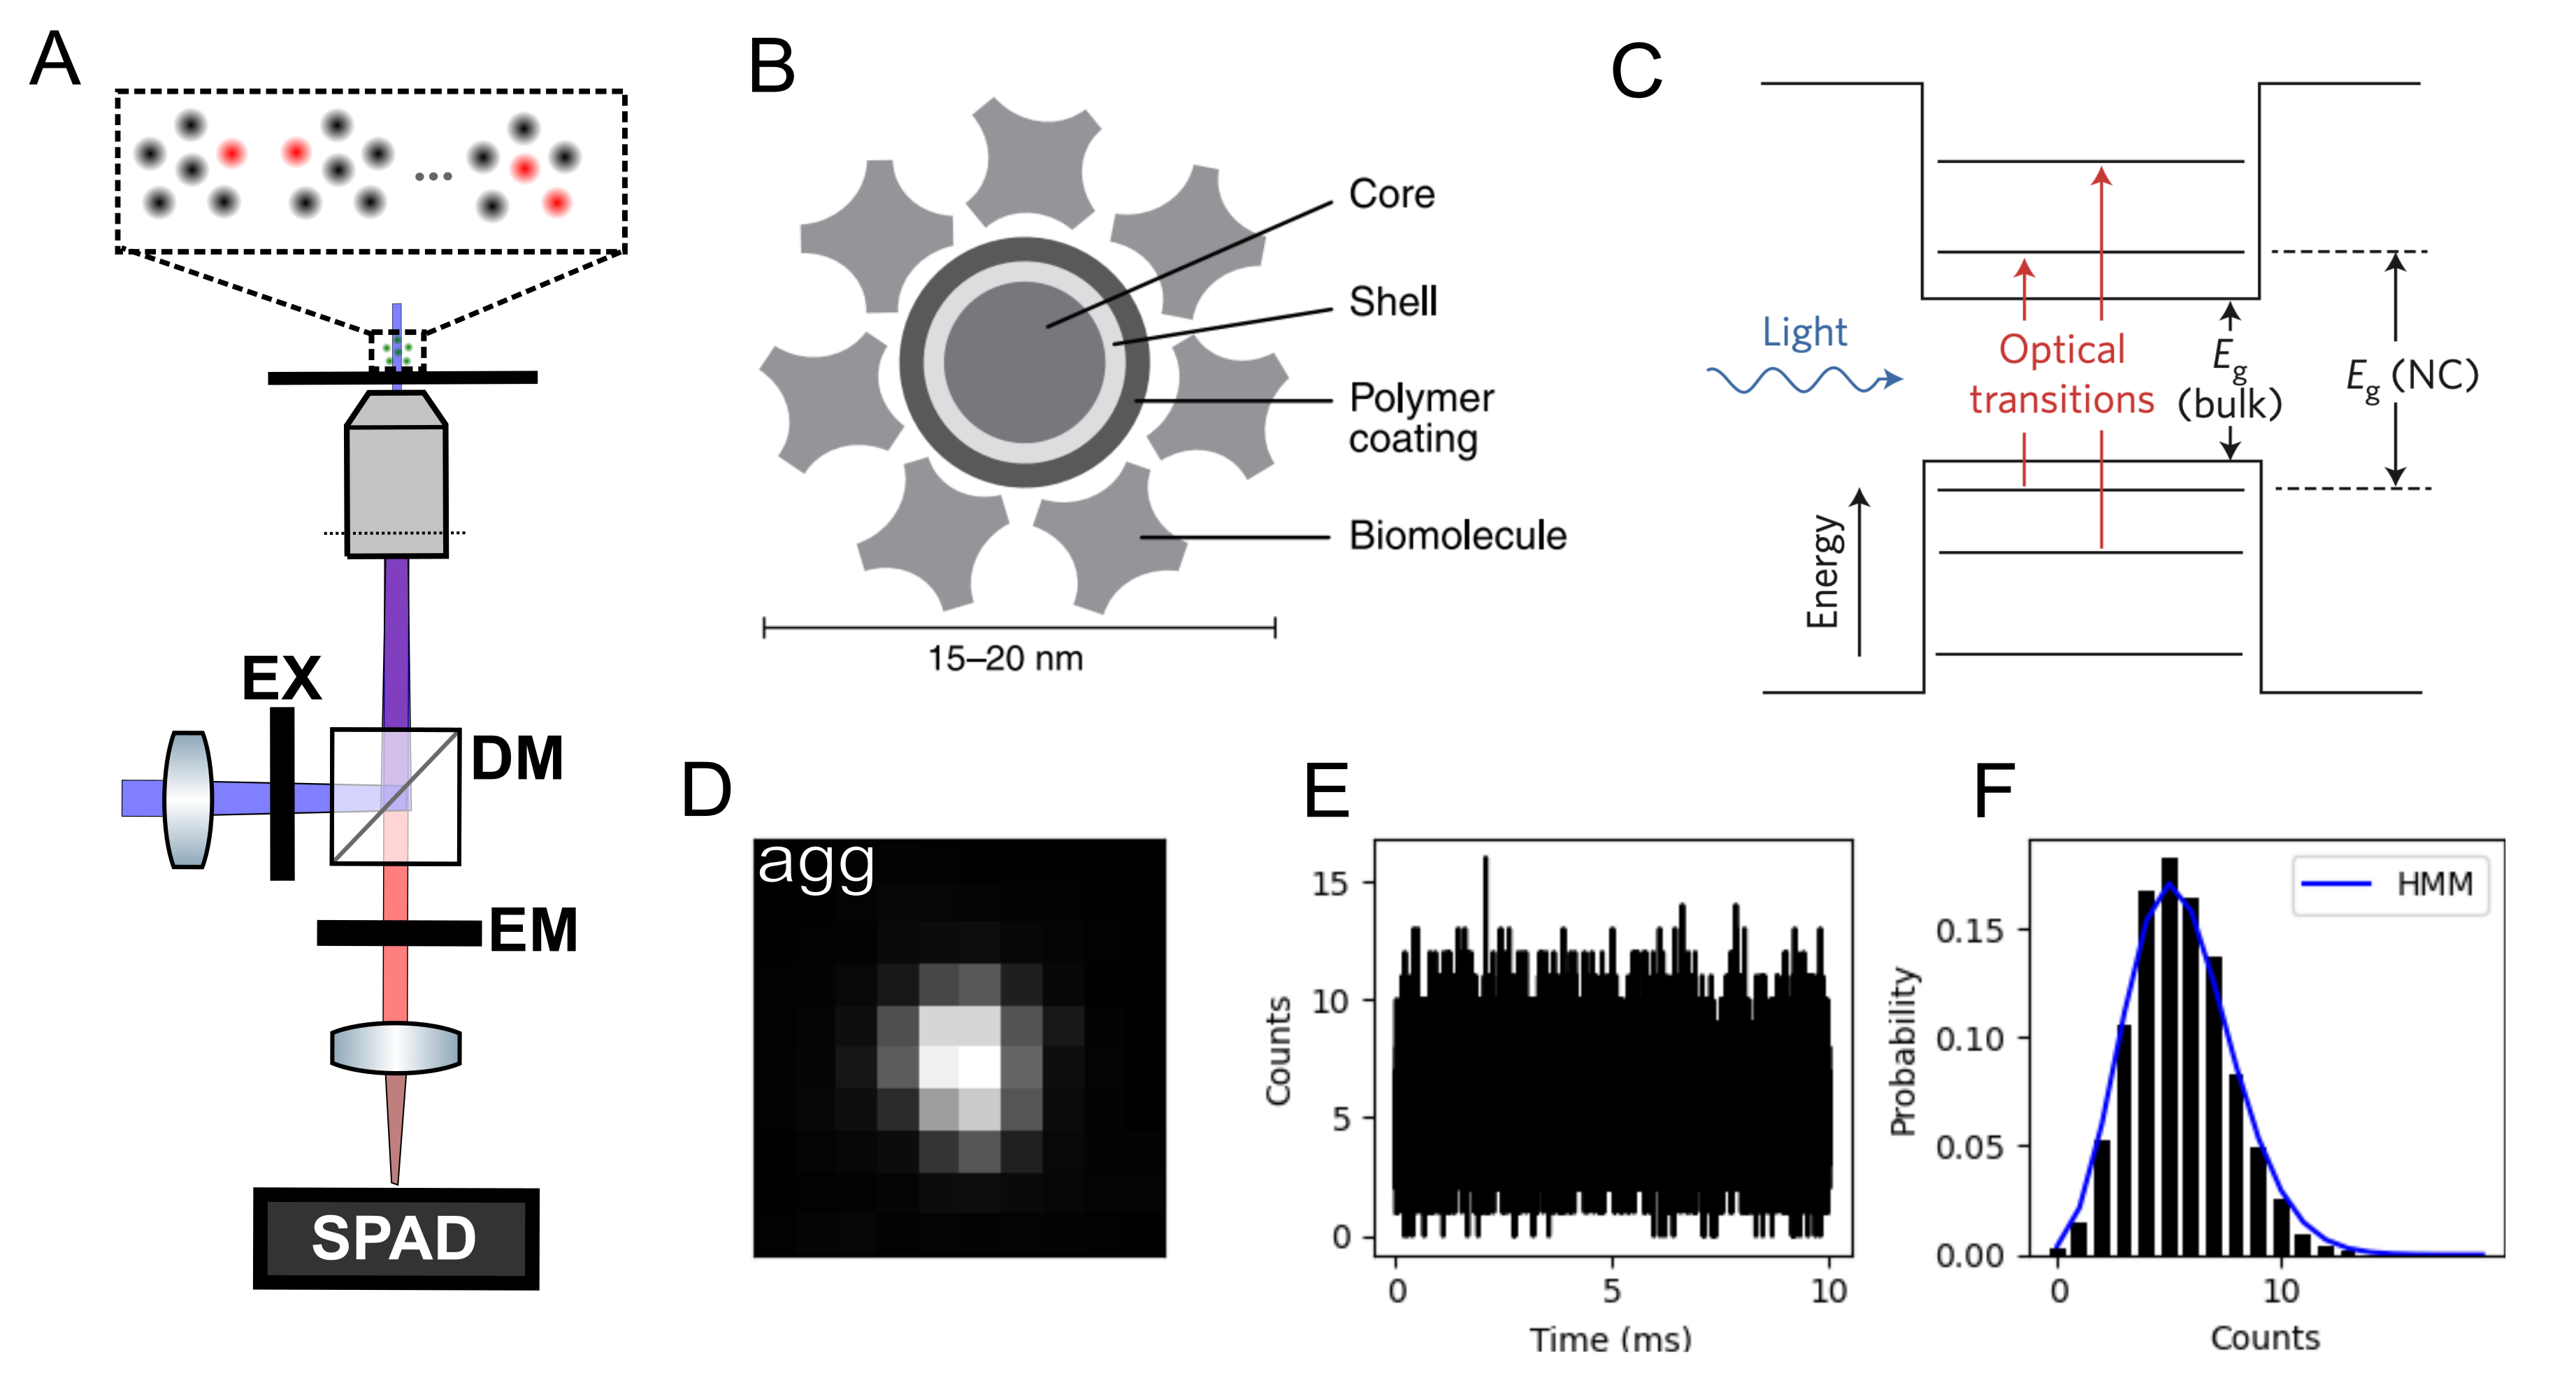
\includegraphics[width=15cm]{QD-Counting.png}
\end{center}
\caption{\textbf{Counting quantum dots with a Hidden Markov Model}}
\end{figure}

\begin{figure}
\begin{center}
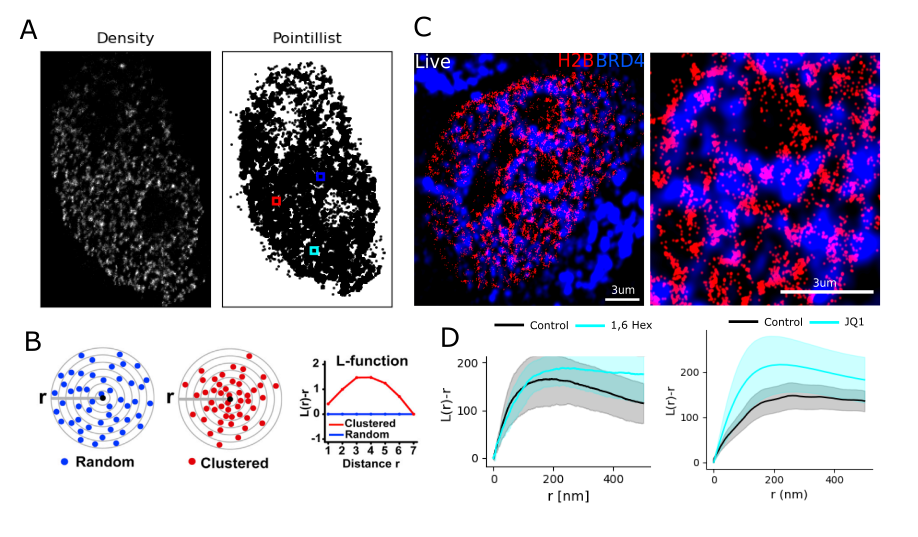
\includegraphics[width=16cm]{BRD4-Results.png}
\end{center}
\caption{\textbf{BRD4 is involved in the maintenance chromatin structure}. (A) Density representation of nucleosome organization using 30nm x 30nm bins and a pointillist representation of nucleosome organization (B) Ripley's K function, Bayesian information criterion (BIC), and log likelihood for a Gaussian mixture model of pointillist localization data of three randomly selected regions of interest. Dashed line drawn at the diffraction limit (C) Localization accumulation over five seconds of imaging time (500 frames) and clustering with DBSCAN for a randomly selected region of interest}
\end{figure}

\subsection{Deep networks outperform MLE in dense localization}

Two major factors contribute to localization errors in SMLM: (i) the noise characteristics of CMOS cameras and (ii) crowding of molecules within a diffraction limited region. Maxmimum likelihood estimation (MLE) is frequently used for isolated molecules and high signal levels, retaining localization errors from 30-40nm (Figure 3c). However, MLE performance tends to degrade in low SNR and dense regimes where the number of emitters within the diffraction limit is greater than one ($K(\lambda/2\mathrm{NA}) > 1$). We employ a convolutional neural network called DeepSTORM, which successively upsamples a monochrome image and outputs a localization map, which can be post-processed to produce molecular coordinates (Figure 2b).  We demonstrate that this architecture can outperform maximum likelhood estimation for all signal levels and molecular densities tested (Figure 2c).




\subsection{Counting quantum dots with a Hidden Markov Model}

Dense aggregates of proteins and nucleic acids with molecular spacing below the diffraction limit are commonplace in the nucleus, creating the need for accurate counting techniques. The ability to accurately count fluorescent emitters using photon statistics has been so far limited to confocal microscopy setups, which are not typically used when imaging dynamics in living cells. As a proof of principle, we imaged organic quantum dots which are a nanocrystal from 15-20nm in size. These nanocrystals are composed of a CdSe semiconductor core, ZnS semiconductor shell, and an amphiphilic polymer coating is applied to confer water solubility and additional functionalization with antibodies, oligonucleotides, etc (Figure 4B). We imaged quantum dots coated on a glass coverslip with a SPAD camera at 1 MHz, and applied our HMM to photon counts from both isolated emitters as well as dense aggregates (Figure 4A,D). Our data indicates that a Poisson HMM models the data well, as measured by the log-likelihood of the sequence of photon counts and distribution of emissions over time (Figure 4E,F). Model selection is carried out purely based on log-likelihood of the sequence.


\begin{comment}
\begin{figure}
\begin{center}
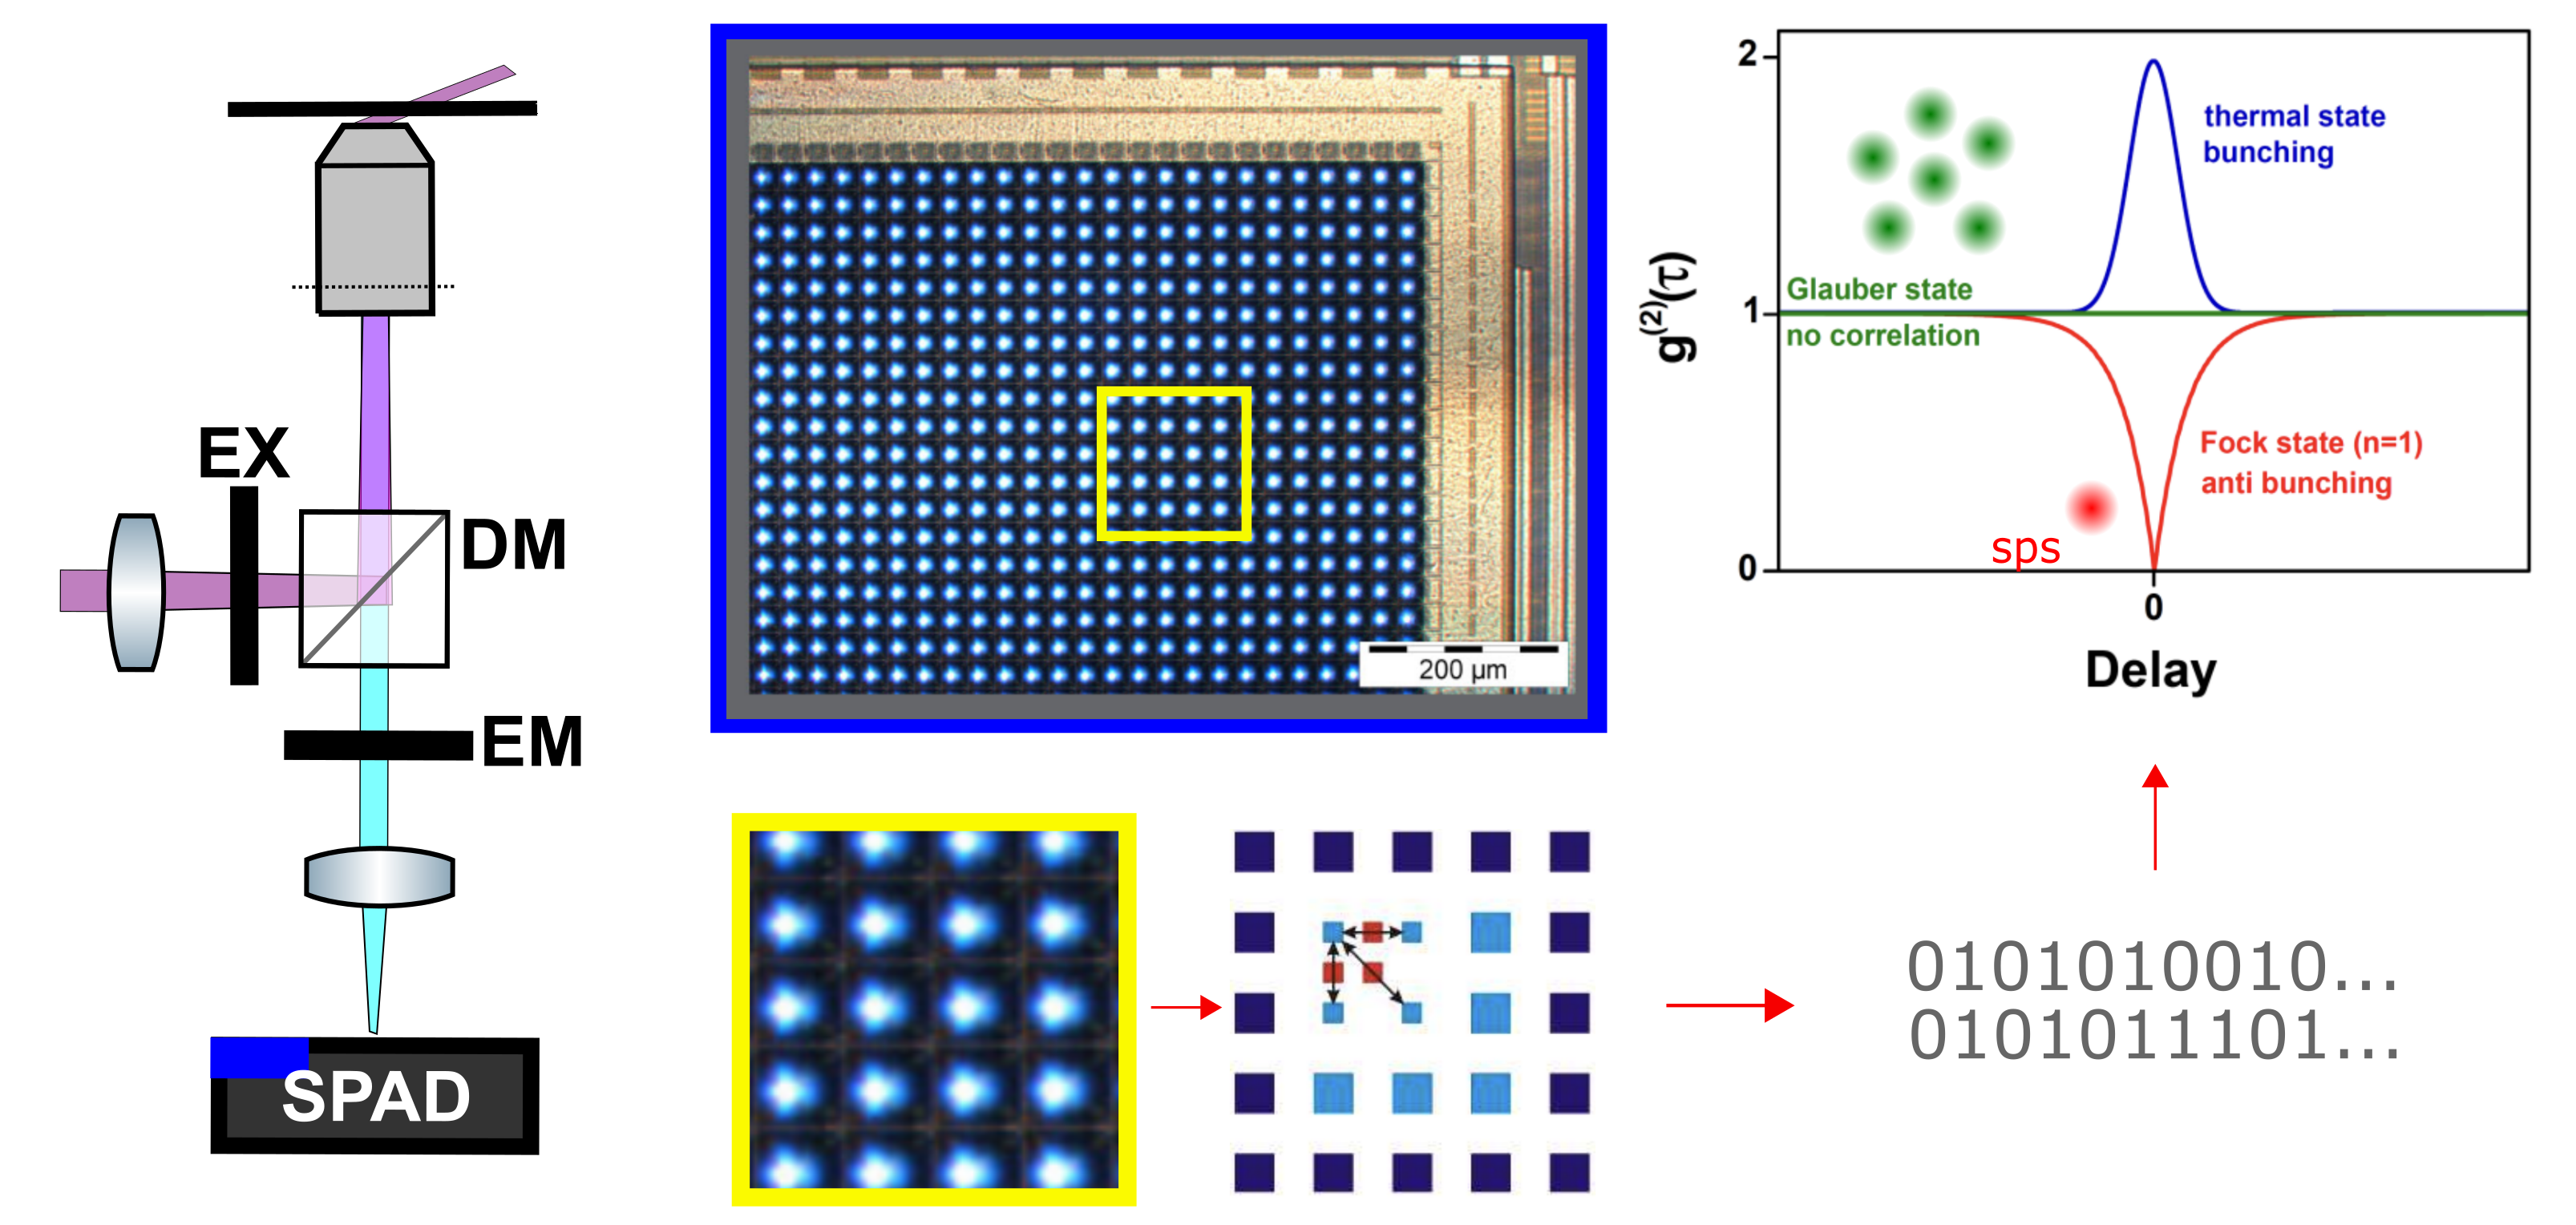
\includegraphics[width=13cm]{Counting.png}
\end{center}
\caption{\textbf{Dense localization with a factorial hidden Markov model} (A) Lateral and axial point spread functions of a single quantum dot at high ($\sim$1.25) and low ($\sim$0.8) numerical aperture (NA). (B) DeepSTORM3D convolutional neural network architecture used for localization. A monochrome image is convolved and upsampled to generate a localization map, which is post-processed to produce a vector of coordinates. (C) Lateral root mean squared error of maximum likelihood estimator (MLE) and a convolutional neural network (CNN) with respect to the incident photon count and the number of molecules within the diffraction limit $\lambda/2\mathrm{NA}$ for high NA. The Cramer-Rao lower bound on lateral uncertainty is shown in gray. Error samples = $10^{3}$}
\end{figure}
\end{comment}


\begin{comment}
To generalize our imaging setup to three-dimensions, we could use that the lateral point spread function has a weak dependence on the axial coordinate (Figure 3a). However, it has been shown that the error around the focus can be large, while negative and positive defocus cannot be distinguished given the symmetric dependence in $z$ (Holtzer 2007). Instead, we choose to introduce astigmatism into the detection path using a weak cylindrical lens (Figure 4a). In effect, this breaks the axial symmetry of the PSF and gives an anisotropic Gaussian which is elongated perpendicular to the optical axis. Localization proceeds by measuring this anisotropy and inverting a model of its axial dependence. At high numerical aperture, a strong dependence of the anisotropy to axial displacement potentially provides more precise three-dimensional localization (Figure 4b). In general, the axial anisotropy can be complex, but is often well described by a polynomial function of the axial displacement (Smith 2010). Unfortunately, astigmatic imaging increases the width of the point spread function significantly, exacerbating localization errors by molecular crowding and low signal to noise ratio. Therefore, we report error statistics for maximum likelihood based methods only, and leave three-dimensional localization with CNNs to future work. As one might expect, at ideal SNR, we show that axial dependence of localization error bears a strong similarity to the axial dependence of the PSF width (Figure 4c). Lateral RMSE can be maintained below 40nm for the anisotropic PSF for $K(\lambda/2\mathrm{NA}) \leq 5$; however, the Jaccard index tends to rapidly degrade at higher molecular densities, making MLE an unsuitable estimator for dense three-dimensional imaging (Figure 5). Three-dimensional single molecule tracking with sparse emitters remains a good application of this method, and will be used in future work.
\end{comment}


\subsection{Super-resolution of nucleosome-BRD4 interactions in living cells}


Here, we use the HaloTag system, a modified haloalkane dehalogenase designed to covalently bind to synthetic ligands  (Los 2008). The HaloTag protein is fused to H2B and is then bound by a rhodomine-derived fluorescent ligands, JF549 or JF646 (Grimm 2015). Two-color imaging of H2B-JF646 and BRD4-GFP showed that BRD4-GFP is present in nucleosome depleted regions, and that BRD4-GFP makes direct contact with the chromatin scaffold (Figure 5C). Exposure of cells to 1,6 Hexanediol promoted an increase in nucleosome cluster sizes, while JQ1 exposure significantly condensed nucleosome clusters (Figure 5D). 

\begin{comment}
\subsection{Inhibition of a super-enhanced gene with JQ1}


The guanylate binding protein (GBP) gene cluster codes for a family of interferon-gamma inducible GTPases. A recent study has confirmed phase separation in the GBP gene family region by co-staining of BRD4 and MED1 marker protein with the GBP gene family region, after infection of macrophages with \emph{Mycobacterium tuberculosis} (Lin 2022). This result is a strong indication that the GBPs gene region tends to relocate into a phase-separated condensate containing BRD4 to efficiently initiate the immune response program. Leveraging previous work on the GBP gene cluster, we (i) confirm the efficacy of JQ1 treatment on GBP5 knockdown after interferon-gamma induction and (ii) determine the effects of JQ1 exposure on BRD4 immunofluorescence signal in Hela nuclei. Fluorescence in-situ hybridization (FISH) demonstrated the formation of GBP5 positive puncta in Hela nuclei after interferon-gamma exposure (Figure 5A-C,F) and mRNA expression over several hours (Figure 5D.) Relief of GBP5 expression was observed by incubating Hela cells for 8h with both interferon-gamma and JQ1 (Figure 5E). BRD4 puncta are abundant in Hela nuclei and exposure of JQ1 for 9h showed a reduction in puncta counts to approximately 70 percent relative to control.
\end{comment}

\section{Discussion and Future Aims}

\subsection{Specific Aim 1: Integrate deep models with counting algorithms for enhanced SMLM}

\subsubsection{Rationale and hypothesis}

We have demonstrated that deep learning algorithms can outperform standard maximum likelihood estimators in low SNR and high density regimes, indicating this is a suitable first step in our SMLM pipeline. In addition, our HMM appears to accurately model the photon detection process. The application of Bayesian methods to prevent overfitting with HMMs is common, and Hierarchical Dirichlet Prior HMM or HDP-HMM may be an appropriate choice in future work. 

\subsubsection{Computational Approach}

Exploration of the high dimensional parameter space in dense STORM is fundamentally intractable. Therefore, the DeepSTORM architecture will be adopted to a probabilistic setting by modifying the output by adding a softmax layer. The arbitrary threshold for Bernoulli probabilities at each pixel conventionally used in DeepSTORM will be removed, and the maximum a posteriori (MAP) number of localizations will be selected from the probability map. Localization uncertainties can then be computed with a Langevin Monte Carlo routine, for fast Bayesian inference. 

\subsection{Specific Aim 2: Determine a role of chromatin architecture in phase separation}

\subsubsection{Rationale and hypothesis}

We have demonstrated by two-color live cell super resolution imaging of H2B and BRD4-GFP that BRD4-GFP protein is present in nucleosome depleted regions in the nucleus. The increase in cluster sizes upon exposure to 1,6 Hexanediol suggests that nucleosome nanodomains may merge after non-specific inhibition of phase separation, while the average spacing of nucleosomes remains. The significant condensation after exposure to JQ1 suggests that BRD4 may be involved in the maintenance of the degree of chromatin condensation, but does not affect the average sizes of nucleosome clusters. Although BRD4-GFP is clearly present in NDRs, there is a significant overlap of H2B and BRD4 signals, leading us to conclude that BRD4 may permeate some nucleosome-dense regions as well. Ultimately, results of treatment of HeLa cells with non-specific and specific phase separation inhibitors suggest that further study into the mechanism of BRD4-specific inhibition with BRD4 silencing and mutation would provide valuable insights into the role of the chromatin scaffold in the formation of transcriptional condensates.

Previous efforts suggest that the acetylated histone reading function of BRD4 is proceeded by recruitment of additional cofactors and chromatin reorganization. Therefore, additional perturbations to BRD4 functions will provide a more complete picture of how BRD4-positive nuclear bodies interact with the chromatin scaffold. Our preliminary data suggests that transcriptional condensates in the nucleus may be stabilized by interactions with neighboring nucleosome clusters. Given that transcriptional condensates associate with accessible DNA, we expect that their depletion by specific inhibition of BRD4 functions will lead to chromatin condensation. Moreover, we expect the action of specific antagonists against BRD4 or its expression will have a distinct effect compared to 1,6 Hexanediol, which may act on the chromatin scaffold directly (Itoh 2021). 


\subsubsection{Experimental Approach}

The chromatin binding modules of BRD4 suggest that phase separated transcriptional condensates in the nucleus are, in part, dependent on nucleosome-BRD4 binding interactions. We propose live-cell super-resolution experiments to determine the nature of the interaction between BRD4 and the chromatin architecture in the formation of BRD4-condensates. To do this, we have first designed siRNAs to knockdown expression of BRD4 protein in HeLa cells, which will determine the effect of global BRD4 loss on chromatin architecture. We will then express wild type and BRD4 mutant plasmids which have mutated Bromodomains. Other experiments may involve mutating the intrinsically disordered regions (IDRs) of BRD4 to impair the phase separation abilities of BRD4. We also address the possibility that small molecule drugs such as JQ1 impact structure of the chromatin scaffold independent of BRD4, we will carry out additional live-cell super-resolution experiments combining BRD4 RNA silencing with JQ1 treatment.


\section{Materials and Methods}

\subsection{Super-resolution imaging of nucleosome nanodomains}

After transient transfection, H2B-Halotag Hela cells were incubated with JF646 HaloTag ligand overnight. Living Hela cells were imaged in a dSTORM photoswitching buffer containing 100mM MEA, 50 ug/ml Glucose Oxidase, and 3.4 mg/ml Catalase (Sigma). Buffer pH was adjusted to ~8 using HCl. Movies were collected using a customized Olympus IX83 microscope equipped with an Olympus 60X 1.25NA oil-immersion objective. Fluorescence images were projected onto an ORCA-Fusion sCMOS camera (Hamamatsu). The microscope was controlled using Micromanager software. JF646 molecules were illuminated with a 640nm laser held at 20mW, as measured at the back focal plane of the objective.  Frames were captured at 100fps.

\subsection{Localization with maximum likelihood estimation}

For each pixel, the number of photoelectrons $S_{k}$ is  multiplied by a gain factor $g_{k} \;[\mathrm{ADU}/e^{-}]$, which generally must be measured during calibration. The readout noise per pixel $\xi_{k}$ is Gaussian with some pixel-specific offset $o_{k}$ (Figure 2a) and variance $\sigma_{k}^{2}$ (Figure 2b). Ultimately, we have a Poisson component of the noise, which scales with the signal level and a Gaussian component, which does not. Therefore, in a single exposure, we measure: 

\begin{equation}
\vec{H} = \vec{S} + \vec{\xi}
\end{equation}

What we are after is the joint distribution $P(\vec{H})$. Fundamental probability theory states that the distribution of $H_{k}$ is the convolution of the distributions of $S_{k}$ and $\xi_{k}$,

\begin{align}
P(H_{k}|\theta) &= P(S_{k})\circledast P(\xi_{k})\\
&= A\sum_{q=0}^{\infty} \frac{1}{q!}e^{-\mu_{k}}\mu_{k}^{q}\frac{1}{\sqrt{2\pi}\sigma_{k}}e^{-\frac{(H_{k}-g_{k}q-o_{k})}{2\sigma_{k}^{2}}}
\end{align}

where $P(\xi_{k}) = \mathcal{N}(o_{k},\sigma_{k}^{2})$ and $P(S_{k}) = \mathrm{Poisson}(g_{k}\mu_{k})$,  $A$ is some normalization constant and $\circledast$ represents convolution. In practice, this expression is difficult to work with, so we look for an approximation. We will use the Poisson-Normal approximation to simplify Eq (4)

\begin{equation*}
\xi_{k} - o_{k} + \sigma_{k}^{2} \sim \mathcal{N}(\sigma_{k}^{2},\sigma_{k}^{2}) \approx \mathrm{Poisson}(\sigma_{k}^{2})
\end{equation*}

Since $H_{k} = S_{k} + \xi_{k}$, we transform $H_{k}' = H_{k} - o_{k} + \sigma_{k}^{2}$, which is distributed according to 

\begin{equation*}
H_{k}' \sim \mathrm{Poisson}(\mu_{k}')
\end{equation*}

where $\mu_{k}' = g_{k}\mu_{k} + \sigma_{k}^{2}$. This result can be seen from the fact the the convolution of two Poisson distributions is also Poisson. The quality of this approximation will degrade with decreasing signal level, since the Poisson distribution does not retain its Gaussian shape at low expected counts. Nevertheless, the quality of the approximation appears to increase exponentially with the expected count, as measured by the Komogonov distance between the convolution distribution (4) and its Poisson approximation (Figure 2c).

Localization microscopy supposes that molecules really do have an exact location in space. In pratice, this is only an approximation since molecules can diffuse at physiological temperatures, and our exposure time would need to tend to zero for this to be exactly true. If we suppose that we can collect a sufficient amount of photons in a short enough time, such that a definite position exists, the following optimization problem is defined

\begin{equation*}
\theta_{\mathrm{MLE}} = \underset{\theta}{\mathrm{argmax}}\prod_{k}P(H_{k}|\theta)= \underset{\theta}{\mathrm{argmin}}-\sum_{k}\log P(H_{k}|\theta)
\end{equation*}


where $\theta_{\mathrm{MLE}}$ represents the maximum likelihood coordinates of a fluorescent molecule. Maximum likelihood estimation (MLE) is a natural choice, since optimization of coordinates under a Poisson likelihood is tractable. Under the Poisson approximation, the model negative log-likelihood is

\begin{align}
\ell(\vec{H}|\theta) &= -\log \prod_{k} \frac{e^{-\left(\mu_{k}'\right)}\left(\mu_{k}'\right)^{n_{k}}}{n_{k}!}\\
&= \sum_{k}  \log n_{k}! + \mu_{k}' - n_{k}\log\left(\mu_{k}'\right)
\end{align}

First order derivatives of the above sum can often be computed analytically, depending on the spatial function $\mu$. The Poisson approximation is also convenient for computing the Fisher information matrix for $\theta_{\mathrm{MLE}}$ and thus the Cramer-Rao lower bound, which bounds the variance of a statistical estimator of $\theta_{\mathrm{MLE}}$, from below (Chao 2016).
Fisher information (separable case): \begin{equation}
I_{ij}(\theta) = \underset{\theta}{\mathbb{E}}\left(\frac{\partial \ell}{\partial\theta_{i}}\frac{\partial\ell}{\partial\theta_{j}}\right) 
\end{equation}

Let $\mu_{k}' = \mu_{k} + \sigma_{k}^{2}$. For an arbitrary parameter,

\begin{align*}
\frac{\partial \ell}{\partial \theta_{i}} &= \frac{\partial}{\partial \theta_{i}} \sum_{k}  x_{k}\log x_{k} + \mu_{k}' - x_{k}\log\left(\mu_{k}'\right)\\
&= \sum_{k} \frac{\partial \mu_{k}'}{\partial\theta_{i}} \left(\frac{\mu_{k}'-x_{k}}{\mu_{k}'}\right)
\end{align*}

\begin{equation*}
I_{ij}(\theta) = \underset{\theta}{\mathbb{E}}\left(\sum_{k}\frac{\partial \mu_{k}'}{\partial\theta_{i}}\frac{\partial \mu_{k}'}{\partial\theta_{j}} \left(\frac{\mu_{k}'-x_{k}}{\mu_{k}'}\right)^{2}\right) = \sum_{k}\frac{1}{\mu_{k}'}\frac{\partial \mu_{k}'}{\partial\theta_{i}}\frac{\partial \mu_{k}'}{\partial\theta_{j}}
\end{equation*}

\subsection{Dense localization with convolutional neural networks}

We employ a localization CNN architecture based on DeepSTORM3D which consists of three main modules. The first module consists of successive dilated convolutions, followed by an upsampling module to increase the lateral resolution by a factor of 4. The third and last module adds additional convolutional blocks to refine localization estimates. This architecture can also be used for three-dimensional localization and thus the final output has $n_{z}$ channels. The final output is followed by an element-wise HardTanh (Maas 2013). A post-processing function $F_{PP}$ uses a user-defined threshold to produce a matrix of coordinates. We find the performance of this architecture on simulated images surpasses MLE, and approaches the Cramer-Rao lower bound at high signal levels, retaining a RMSE near 20nm for $K(\lambda/2\mathrm{NA}) \leq 5$, at high signal levels (Figure 3c). 

\subsection{Hidden Markov Model for counting fluorescent emitters}

\subsection{Computation of Ripley's L-function}

%\subsection{Uncertainty quantification with Markov Chain Monte Carlo}
%To filter out suspicious localizations, we used Metropolis-Hastings Markov Chain Monte Carlo (MCMC) to estimate the posterior %marginals on coordinates. MCMC is asymptotically exact, which is not guaranteed by variational methods which may rely on a Laplace %approximation around the MLE. Metropolis-Hastings is run for 3000 iterations, the first half is discarded as burn-in. A proposal $%\theta' = \theta + \xi$ was generated with $\xi\sim \mathcal{N}(0,\sigma^{2}I)$ where $\sigma^{2}=0.01$. The acceptance probability is%
%\begin{equation*}
%\alpha = e^{\beta(\ell(\theta)-\ell(\theta'))}
%\end{equation*}
%with $\beta=5$ to achieve a target acceptance rate of $0.3$. Localizations with uncertiainty exceeding 50nm are removed from the %dataset.

%\subsection{Gaussian mixture model for correcting localization artifacts}

%In high duty cycle SMLM, the sample molecule can be localized several times throughout an imaging acqusition. We take a probabilistic %approach, motivated by Occam's razor, assuming stationary conditions in the sample. The localization data is used to construct a %Gaussian mixture model (Bishop 2006) with one Gaussian mode per localization, parameterized by posterior variances. These can be %computed with MCMC, but for simplicity we replace them by the expected variance $\Sigma_{0}$. We then compute the distance matrix %$D_{ij}$ between all localizations and iteratively selects the nearest pair of coordinates and fuses them by replacement with their %average position: $\mu_{1},\mu_{2}\rightarrow \mu=\frac{\mu_{1}+\mu_{2}}{2}$ and covariance $\Sigma_{0}$. After each fusion, we %compute the Bayesian information criterion (BIC): 

%\begin{equation*}
%\mathrm{BIC} = k\ln(n) - 2\ln (\mathcal{L})
%\end{equation*}

%where $n$ is the number of localizations, $k=2n$ is the number of parameters in the GMM, and $\mathcal{L}$ is the data likelihood. We %compute the model log-likelihood

%\begin{equation*}
%\ell(\theta|\bm{r}) = \sum_{n}\pi_{n}\mathcal{N}(\bm{r}_{n},\Sigma_{0})
%\end{equation*}

%Iteration then proceeds to minimize the BIC.

\subsection{Fourier Ring Correlation}

Following (Nieuwenhuizen 2013), a pair of subsets is drawn from the full list of localizations, and isotropic Gaussian kernel density estimation is performed. The Fourier Ring Correlation is calculated as a function of the ring radius $q$ for two images $f_{1}$ and $f_{2}$

\begin{equation*}
\mathrm{FRC}(q) = \frac{\sum_{\vec{q}\in\mathrm{circle}}\tilde{f_{1}}(\vec{q})\tilde{f_{2}}(\vec{q})^{*}}{\sqrt{\sum_{\vec{q}\in\mathrm{circle}}|f_{1}(\vec{q})|^{2}}\sqrt{\sum_{\vec{q}\in\mathrm{circle}}|f_{2}}(\vec{q})|^{2}}
\end{equation*}

where $\tilde{f_{1}}$ is the discrete Fourier transform of $f_{1}$.

\begin{comment}
\subsection{Cell culture, transfection, and treatments}

Hela cells were cultured in DMEM supplemented with 10 percent fetal bovine serum (Gibco) at 37C, 5  percent  CO2 in a humidified incubator. For super-resolution experiments, cells were seeded in a 35mm FluoroDish (WPI), and transiently transfected with pBREBACK-H2BHalo plasmid (Addgene plasmid 91564) using Lipofectamine 3000 (ThermoFisher). For immune activation, cells were incubated with 50ng/ml Interferon-gamma (Gibco), diluted in fresh DMEM. BRD4 inhibition with JQ1 (Chemie Tek) was carried out using specified concentrations and incubation time in fresh DMEM.  

\subsection{RNA fluorescence in-situ hybridization}

Cells were seeded in 8-well chamber slides with 1.5 glass coverslip bottom (Ibidi). GBP5 expression was induced with 50ng/ml Interferon-gamma, followed by fixation. Stellaris RNA FISH Wash Buffer A (Biosearch Technologies, Inc., SMF-WA1-60), 10  percent  Deionized Formamide (EMD Millipore, S4117) in RNase-free water (Life Technologies, AM9932) for 5 min at RT. Cells were hybridized with 90  percent  Stellaris RNA FISH Hybridization Buffer (Biosearch Technologies, SMF-HB1-10), 10  percent  Deionized Formamide, 12.5 µM Stellaris RNA FISH probes designed to hybridize introns of the . Hybridization was performed in a humidified chamber at 37C. Cells were then washed with Wash Buffer A for 30 min at 37°C and nuclei were stained with 15ng/ml DAPI in Wash Buffer A for 5 min at RT. After one 5-min was with Stellaris RNA FISH Wash Buffer B (Biosearch Technologies, SMF-WB1-20) at RT. Images were acquired as 10x10 grids on an ASI RAMM widefield microscope with 60X 1.4NA Nikon oil-immersion objective using Micromanager acquisition software and a Hammamatsu ORCA-Flash4.0v3 camera.  

RNA FISH probes were designed and generated by Biosearch Technologies Stellaris RNA FISH to target exons of GBP5. 

\subsection{Immunofluorescence}

Cells grown in chamber slides or 35mm dishes and permeabilized with 0.3  percent  (v/v) Triton-X100 (Sigma-Aldrich) in PBS and blocked for 1h in 5  percent  (w/v) nonfat dry milk at 4C. Cells were incubated overnight at 4C using primary antibody anti-BRD4 (Cell Signaling, clone E2A7X; 1:1000). Secondary antibodies for BRD4 (Cell Signaling Anti-Rabbit igG-Alexa488, 1:1000). 

\subsection{Quantitative reverse transcription polymerase chain reaction}

GBP5 induction was validated with RT-qPCR, using the TaqMan gene expression assay. Cell culture followed standard procedure, followed by homogenization with lysis buffer with 2-mercaptoethanol (Bio-Rad). Suspension was vortexed and transferred into a clean RNase-free tube. The homogenate was centrifuged at 12,000g for 2 minutes. RNA was purified using PureLink RNA Mini Kit (Invitrogen) and stored on ice. Reverse transcription was carried out using the iScript Advanced cDNA Synthesis Kit (Bio-Rad).Taqman probes were designed against GAPDH and GBP5 genes, and RT-qPCR was run in a 96 well plate on a qPCR machine (Applied Biosystems). Relative RNA level of GBP5 to GAPDH were computed using the $\Delta\Delta C_{t}$ method (Schmittgen 2008). 

\subsection{Immunoblotting}

Cells were washed and lysis buffer added (RIPA buffer: PMSF: protease inhibitor cocktail: orthovanadate=100:1:1:1). Cells were then scraped and sonicated for 15 seconds using an ultrasonic homogenizer. Lysate was centrifuged at high speed (13200r/min) for 10-15 minutes at 4C to pellet the cellular debris. Total protein concentration was determined by a BCA Protein Assay Kit (Pierce). For electrophoresis, protein samples were prepared according to a protein-loading ratio of 3:1. Sample was mixed and heated at 95℃ for 5 min, followed by vortex and centrifuge. After running the gel, it was removed from the cassette and assembled inside the Trans-Blot Turbo Transfer System cassette. Transfer was run at 2.5A for 7min. Sample was then blocked using 5  percent  skim milk blocking solution prepared with PBST. Primary GBP5 antibody was diluted with PBST (1:1000) and incubated at 4C overnight. The secondary antibody was diluted with PBST (1:2000) and placed on a rocker and incubate at RT for 45min. Western blots on PVDF membranes were scanned using the Odyssey fluorescence scanning system software. 
\end{comment}

\section{Supplemental Information}

\begin{comment}

\begin{figure}
\begin{center}
\includegraphics[width=16cm]{GBP5.png}
\end{center}
\caption{\textbf{Inhibition of a BRD4-controlled gene with JQ1}. (A) Putative GBP5 transcription sites at the specified time points following IFN-$\gamma$ exposure. (B,C) High resolution zoom of GBP5 in-situ hybridization 8 hours folowing IFN-$\gamma$ exposure (D) Induction of GBP5 expression in Hela cells following IFN-$\gamma$ exposure, measured with RT-qPCR (E) Knockdown of GBP5 expression 8 hours folowing IFN-$\gamma$ exposure with 1uM JQ1 treatment ($n=3$,$** P < 0.01$) (F) Western blot of GBP5 protein expression following IFN-$\gamma$ exposure (G) BRD4 immunofluorescence 9h after first exposure to (+)JQ1 (H) Ratio of BRD4 puncta count 9h after JQ1 exposure relative to control ($n=108$,$** P < 0.001$)}
\end{figure}
\end{comment}

%\begin{figure}
%\begin{center}
%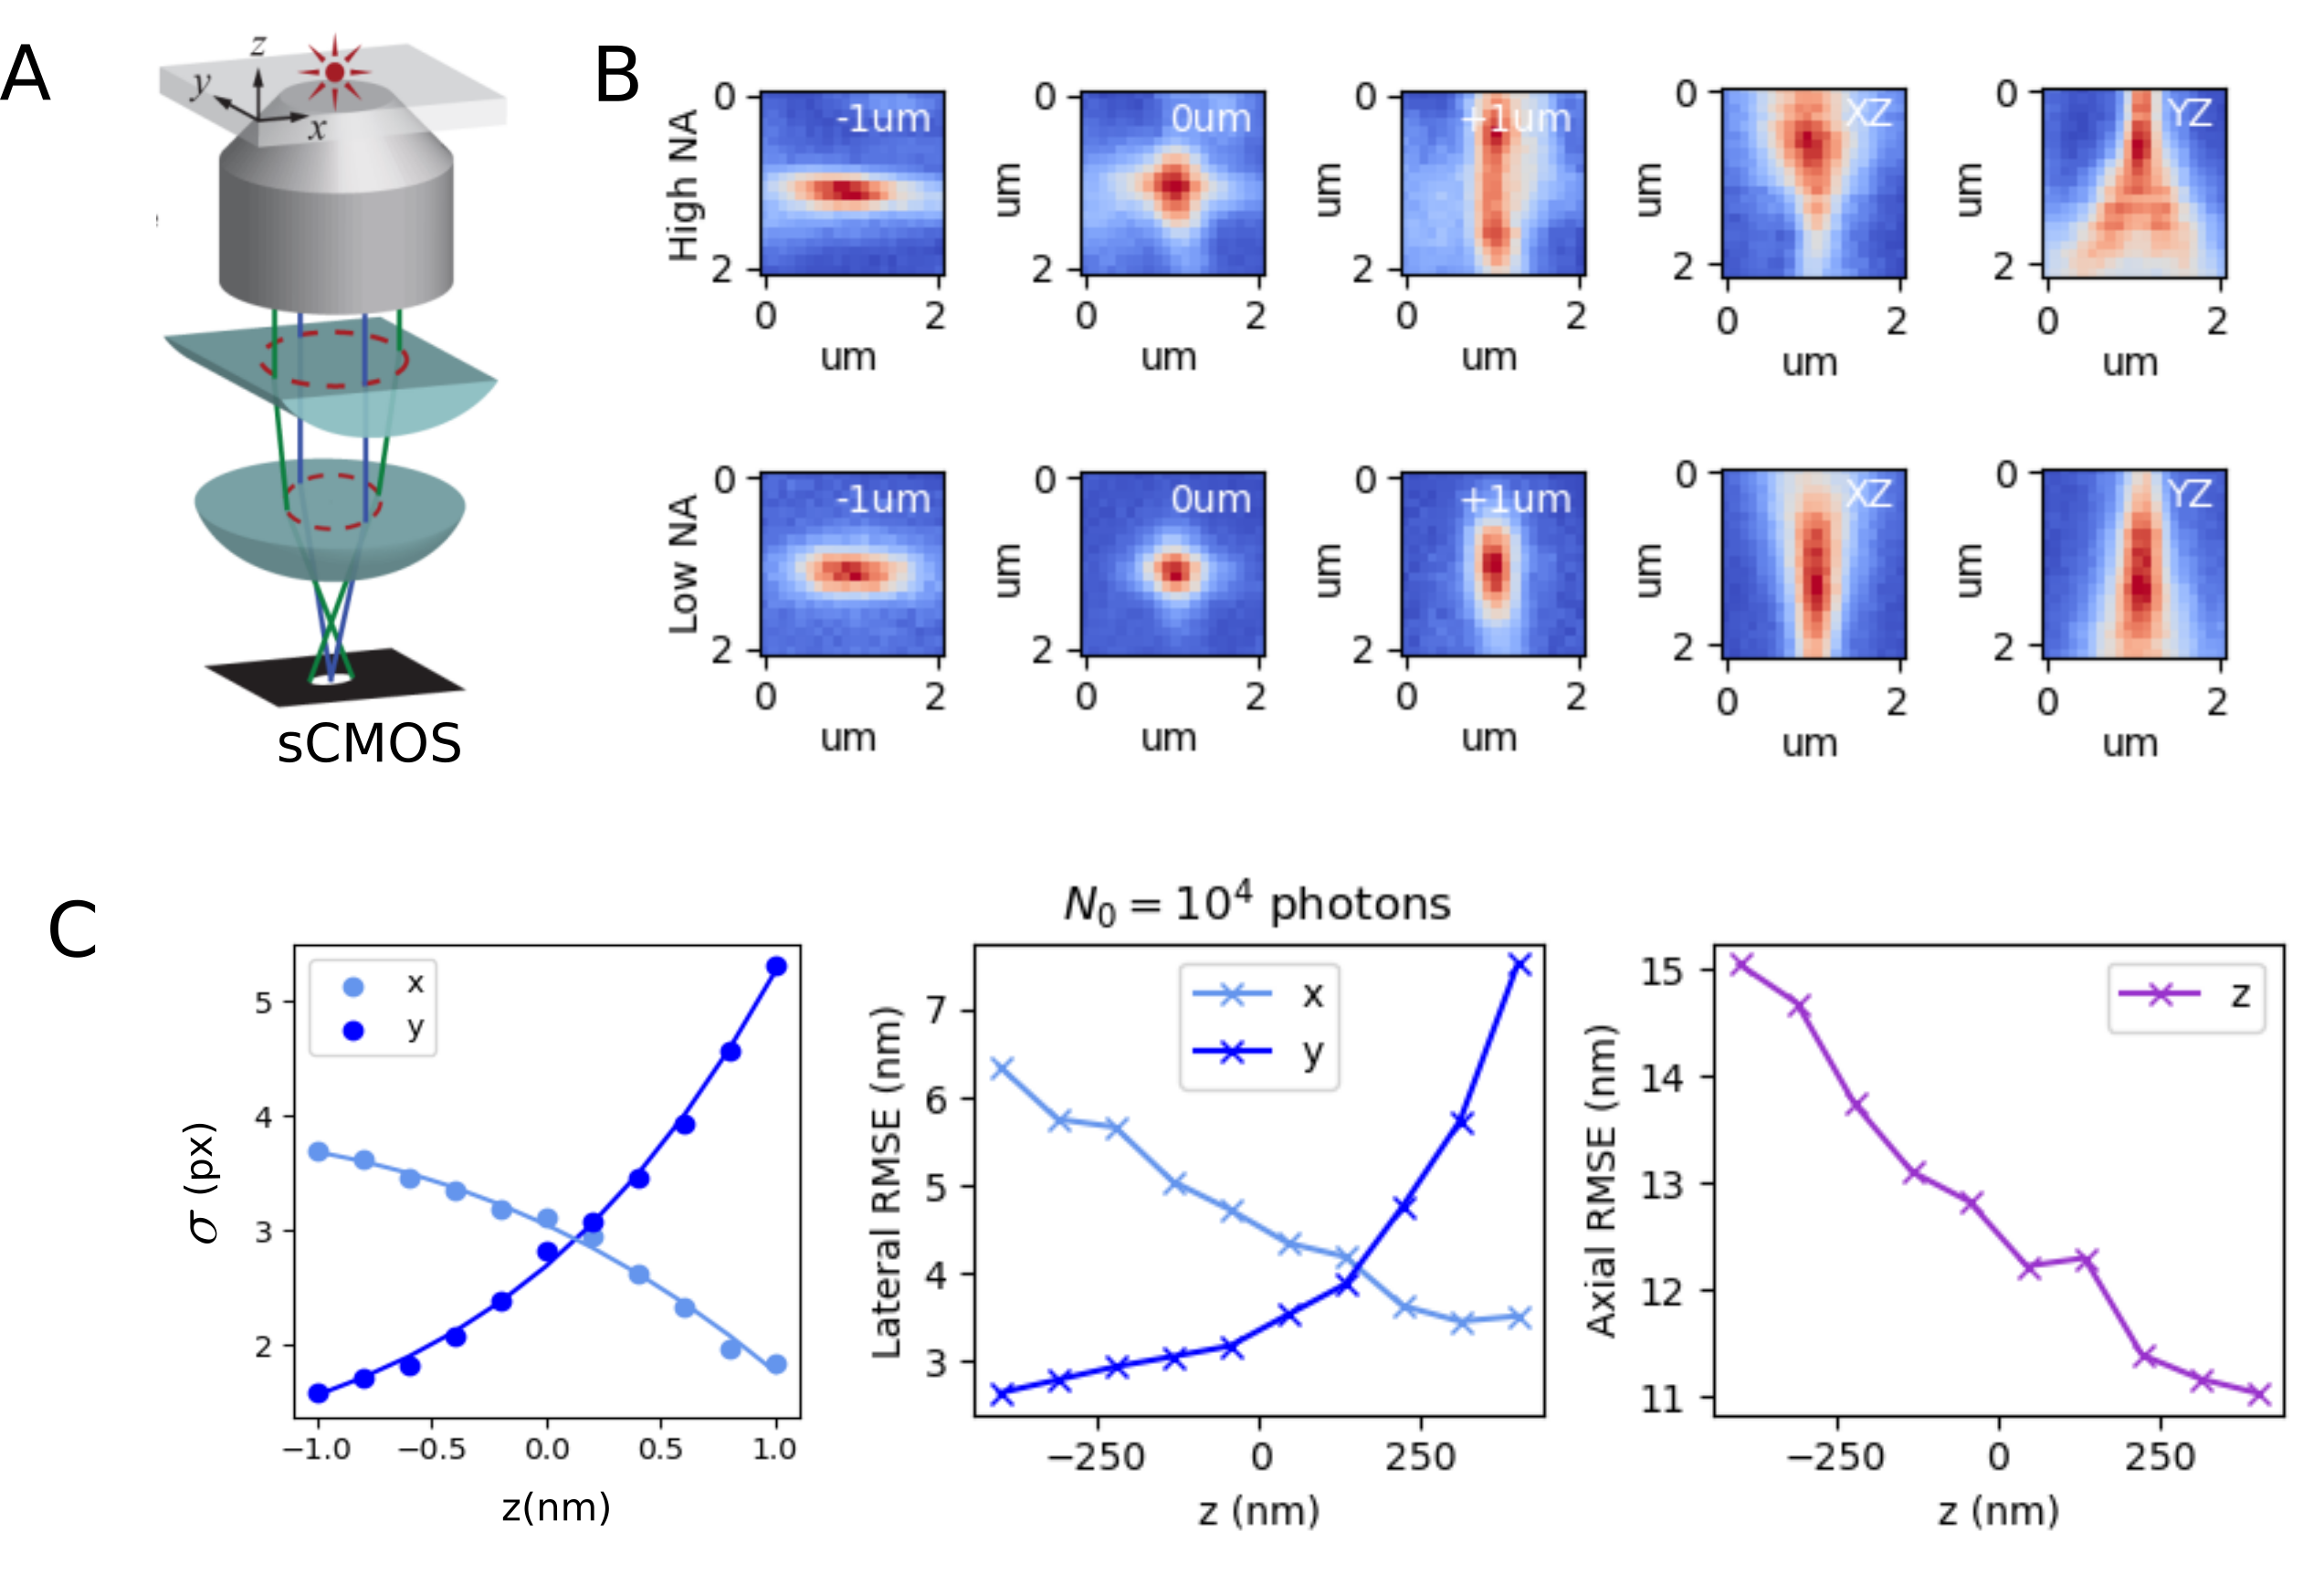
\includegraphics[width=14cm]{Astigmatism.png}
%\end{center}
%\caption{\textbf{Axial precision for three-dimensional localization at ideal SNR} (A) Simplified lens relay for astigmatic imaging of %a fluorescent emitter using a weak cylindrical lens ($f$=10m). (B) Lateral and axial point spread function of a single quantum dot on %a 1.5 glass coverslip for high ($\sim$1.25) and low ($\sim$0.8) numerical aperture (NA). (C) Polynomial fit of the standard deviation %of the lateral point spread function along orthogonal axes (left) Root mean squared error (RMSE) of lateral coordinates as a function %of the axial coordinate, using simulated images fit with MLE (middle). RMSE of the axial coordinate, using simulated images fit with %MLE (right). Error samples = $10^{3}$}
%\end{figure}




\begin{figure}
\begin{center}
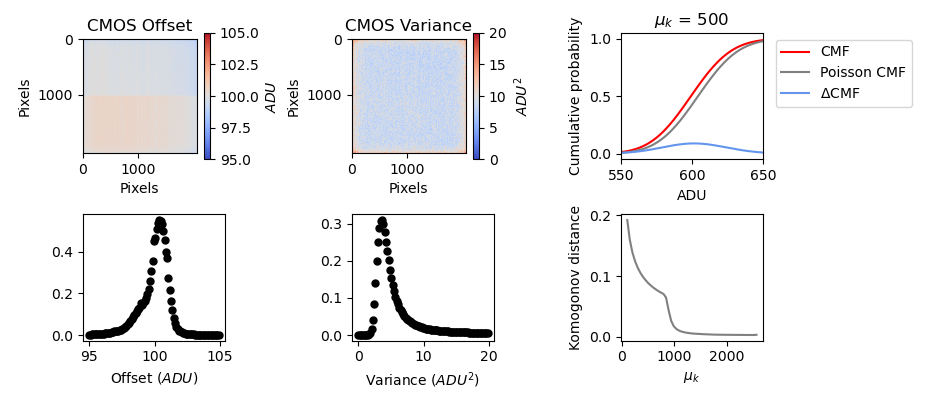
\includegraphics[width=16cm]{Noise.png}
\end{center}
\caption{\textbf{Classical emission statistics of fluorescent markers}. (A) Offset for zero incident photons (B) Variance for zero incident photons (C) Cumulative mass function for the convolution distribution and its Poisson approximation for rate parameter $\mu_{k} = 500$ counts (D) Komogonov distance measured as a function of rate parameter $\mu_{k}$}
\end{figure}

\begin{figure}
\begin{center}
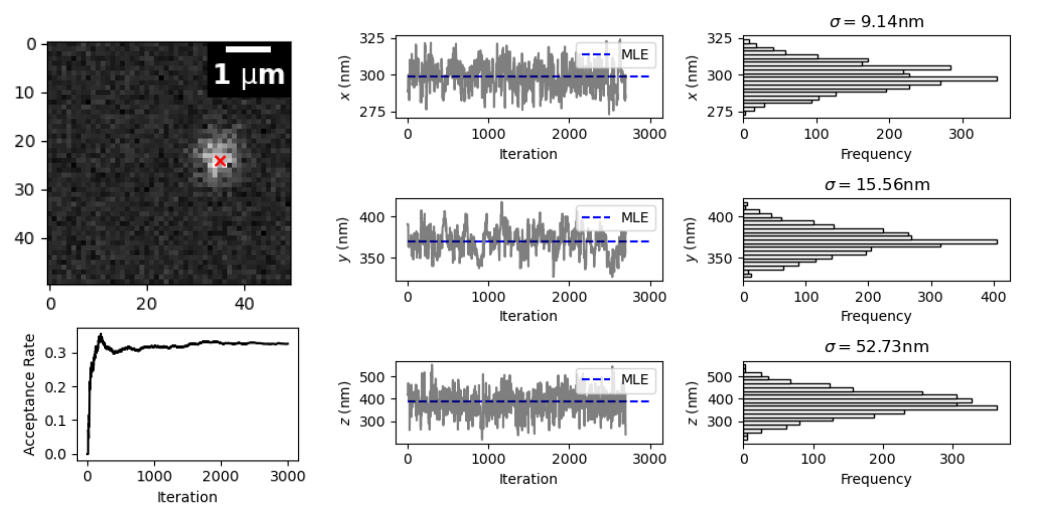
\includegraphics[width=16cm]{MCMC.png}
\end{center}
\caption{\textbf{Computing epistemic uncertanties with Metropolis-Hastings}. (top left) Simulated point spread function for $N_{0}=10^{3}$ photons with a red x at $x_{\mathrm{MLE}}$ and $y_{\mathrm{MLE}}$ (bottom left) Acceptance rate of Markov chain (middle) Markov chains sampling from the posterior distribution on molecule coordinates in 3D, with the maximum likelihood estimation in dashed blue (right) Estimated posterior marginals on the localization parameters with their respective uncertanties}
\end{figure}

\begin{figure}
\begin{center}
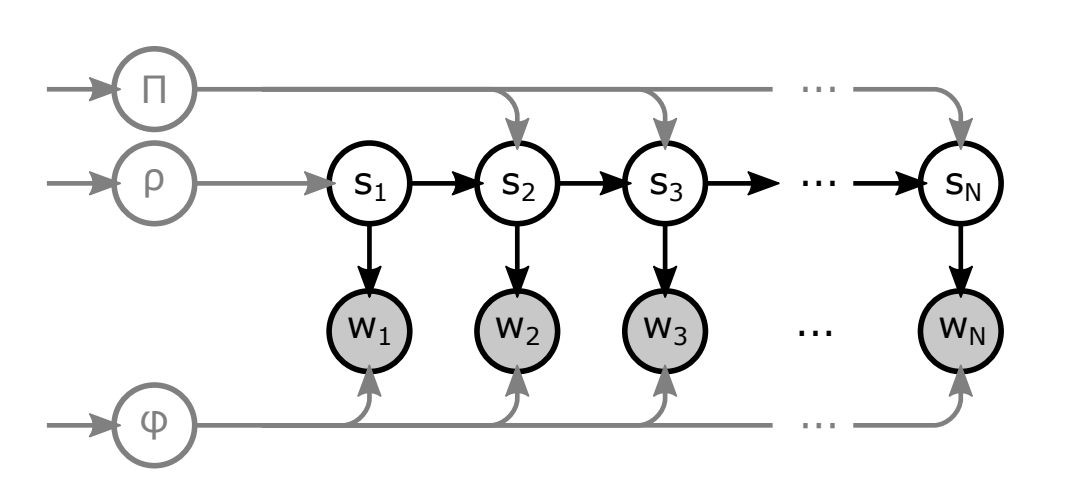
\includegraphics[width=14cm]{HMM.png}
\end{center}
\caption{\textbf{Graphical representation of Hidden Markov Model (HMM) for counting QDs} See main text for full description}
\end{figure}


%\begin{figure}
%\begin{center}
%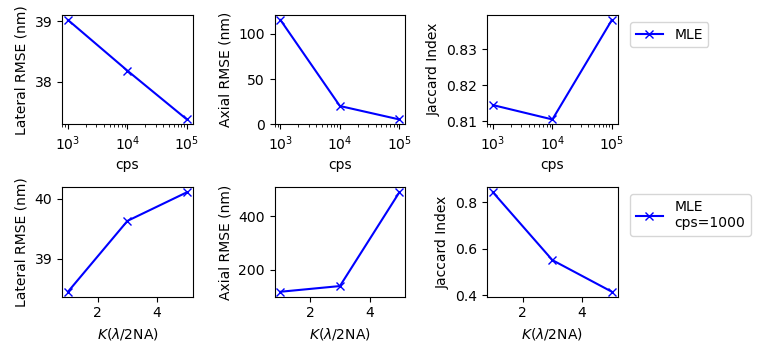
\includegraphics[width=16cm]{PSF3D.png}
%\end{center}
%\caption{\textbf{Dependence of axial and lateral precision on SNR and molecular density}. (upper row) Lateral and axial root mean %squared errors (RMSE) at varying signal levels (lower row) Lateral and axial RMSE for varying molecule counts within a diffraction %limit radius for $10^{3}$ photon counts. Error samples = $10^{3}$}
%\end{figure}

\subsection{Estimator precision sets the resolution limit in localization microscopy}

Complementary Metal-Oxide-Semiconductor (CMOS) cameras have become a central tool in fluorescence microscopy. The CMOS sensor is revered for its high frame rates, allowing researchers to reach higher temporal resolutions. Nevertheless, CMOS cameras have noise sources intrinsic to their operation, such as shot noise and readout noise. The former phenomenon can describe a superposition of processes; namely, the fluctuations of the number of photons due to the quantum nature of light, and the random conversion of photons into photoelectrons within the semiconductor material with a quantum efficiency below unity. Here we will often refer to the photon count $N_{0}$, which has a determined value, rather than being described by statistically. The \emph{measured} photon count, however, is well-described by a Poisson process (Schottky 1918). A shot-noise limited image with $N$ pixels is then described as a family of Poisson variables, with units of photoelectrons


\begin{equation}
\vec{S} = \left[\mathrm{Poisson}(\mu_{1}), \mathrm{Poisson}(\mu_{2}), ..., \mathrm{Poisson}(\mu_{N})\right]
\end{equation}

CMOS sensors also suffer from other noise sources, such as readout noise or dark current, resulting in a nonzero signal even in the absence of incident light. Dark current is due to statistical fluctuations in the photoelectron count within a semiconductor material in thermal equilibrium. Fortunately, these additional noise sources are governed by the central limit theorem, and can be efficiently summarized as the component of the noise which exhibits a Gaussian distribution. Readout noise has been often neglected in localization algorithms because its presence in EMCCD cameras is small enough that it can be ignored within the tolerances of the localization precision. In the case of high speed CMOS cameras, however, the readout noise of each pixel is significantly higher and, in addition, every pixel has its own noise and gain characteristic sometimes with dramatic pixel-to-pixel variations (Huang 2013). Therefore, accurate localization and simulation necessisitates models which incorporate detailed sensor properties. 


\subsection{Integrated isotropic and anisotropic Gaussian point spread functions}

For the sake of simplicity, it is common to describe the point spread function (PSF) as a two-dimensional isotropic Gaussian (Zhang 2007). This is an approximation to the more rigorous models given by Richards and Wolf (1959) or Gibson and Lanni (1989). 

\begin{equation*}
\mathrm{G}(x,y) = \frac{1}{2\pi\sigma^{2}}e^{-\frac{(x-x_{0})^{2}+(y-y_{0})^{2}}{2\sigma^{2}}}
\end{equation*}

The chracteristic width $\sigma$ of the PSF typically depends on the numerical aperture of the objective lens and The image of a fluorescent molecule captured by the objective lens, can be thought of as two-dimensional histogram of photon arrivals and a discretized form of the classical intensity profile $\mathrm{G}(x,y)$. The value at a pixel approaches an integral of this density over the pixel:

\begin{equation}
\mu_{k} = i_{0}\lambda_{k} = i_{0}\int_{\mathrm{pixel}} G(x,y)dxdy
\end{equation}

where $i_{0} = g_{k}\eta N_{0}\Delta$. The parameter $\eta$ is the quantum efficiency and $\Delta$ is the exposure time. $N_{0}$ represents the number of photons emitted per unit time. The above integral can be expressed in terms of error functions, and the full calculation can be found in (Smith 2010). 

\section{References}

\noindent [1] Schermelleh, L. et al. Super-resolution microscopy demystified. Nature Cell Biology vol. 21 72–84 (2019). 
\newline
\noindent [2] Speiser, A. et al. Deep learning enables fast and dense single-molecule localization with high accuracy. Nat Methods 18, 1082–1090 (2021).
\newline
\noindent [5] Dertinger, T., Colyer, R., Iyer, G., Weiss, S. Enderlein, J. Fast, background-free, 3D super-resolution optical fluctuation imaging (SOFI). PNAS
\newline
\noindent [6] Richards, B. Wolf, E. Electromagnetic Diffraction in Optical Systems. II. Structure of the Image Field in an Aplanatic System. Source: Proceedings of the Royal Society of London. Series A, Mathematical and Physical Sciences vol. 253 (1959). 
\newline
\noindent [8] Ouyang, W., Aristov, A., Lelek, M., Hao, X. Zimmer, C. Deep learning massively accelerates super-resolution localization microscopy. Nat Biotechnol 36, 460–468 (2018). 
\newline
\noindent [10] Chao, J., Sally Ward, E. Ober, R. J. Fisher information theory for parameter estimation in single molecule microscopy: tutorial. Journal of the Optical Society of America A 33, B36 (2016). 
\newline
\noindent [12] Nehme, E. et al. DeepSTORM3D: dense 3D localization microscopy and PSF design by deep learning. Nat Methods 17, 734–740 (2020). 
\newline
\noindent [35] Nieuwenhuizen, R et al. Measuring image resolution in optical nanoscopy. Nature Methods 10. 557-562 (2013). 
\noindent [15] Tokunaga, M., Imamoto, N. Sakata-Sogawa, K. Highly inclined thin illumination enables clear single-molecule imaging in cells. Nat Methods 5, (2007). 
\newline
\noindent [16] Kalisvaart, D. et al. Precision in iterative modulation enhanced single-molecule localization microscopy. Biophys J 121, 2279–2289 (2022). 
\newline
\noindent [17] Zhang, B., Zerubia, J. Olivo-Marin, J.-C. Gaussian approximations of fluorescence microscope point-spread function models. (2007). 
\newline
\noindent [24] Smith, C. S., Joseph, N., Rieger, B. Lidke, K. A. Fast, single-molecule localization that achieves theoretically minimum uncertainty. Nat Methods 7, 373–375 (2010). 
\newline
\noindent [25] Sabari, B. R. et al. Coactivator condensation at super-enhancers links phase separation and gene control. Science (1979) 361, (2018). 
\newline
\noindent [26] Linde, S. Van De et al. Direct stochastic optical reconstruction microscopy with standard fluorescent probes. Nat Protoc 6, 991–1009 (2011). 
\newline
\noindent [27] Huang, F. et al. Video-rate nanoscopy using sCMOS camera-specific single-molecule localization algorithms. Nat Methods 10, 653–658 (2013). 
\newline
\noindent [29] Hnisz, D., Shrinivas, K., Young, R. A., Chakraborty, A. K. Sharp, P. A. A Phase Separation Model for Transcriptional Control. Cell vol. 169 13–23 (2017). 
\newline
\noindent [30] Grimm, J. B. et al. A general method to improve fluorophores for live-cell and single-molecule microscopy. Nat Methods 12, 244–250 (2015). 
\newline
\noindent [31] Nozaki, T. et al. Dynamic Organization of Chromatin Domains Revealed by Super-Resolution Live-Cell Imaging. Mol Cell 67, 282-293.e7 (2017). 
\newline
\noindent [32] Xu, J. et al. Super-Resolution Imaging of Higher-Order Chromatin Structures at Different Epigenomic States in Single Mammalian Cells. Cell Rep 24, 873–882 (2018). 
\newline
\noindent [33] Boettiger, A. N. et al. Super-resolution imaging reveals distinct chromatin folding for different epigenetic states. Nature 529, 418–422 (2016). 
\newline
\noindent [34] Nozaki, T. et al. Dynamic Organization of Chromatin Domains Revealed by Super-Resolution Live-Cell Imaging. Mol Cell 67, 282-293.e7 (2017). 
\noindent [3] Barth, R., Bystricky, K. Shaban, H. A. Coupling chromatin structure and dynamics by live super-resolution imaging. Sci. Adv vol. 6 (2020). 
\newline
\noindent [7] Devaiah, B. N. et al. BRD4 is a histone acetyltransferase that evicts nucleosomes from chromatin. Nat Struct Mol Biol 23, 540–548 (2016). 
\newline
\noindent [9] Filippakopoulos, P. et al. Selective inhibition of BET bromodomains. Nature 468, 1067–1073 (2010). 
\newline
\noindent [10] Grimm, J. B. et al. A General Method to Improve Fluorophores Using Deuterated Auxochromes. JACS Au 1, 690–696 (2021). 
\newline
\noindent [13] Itoh, Y. et al. 1,6-hexanediol rapidly immobilizes and condenses chromatin in living human cells. Life Sci Alliance 4, (2021). 
\newline
\noindent [14] Han, X. et al. Roles of the BRD4 short isoform in phase separation and active gene transcription. Nat Struct Mol Biol 27, 333–341 (2020). 
\newline
\noindent [18] Los, G. V. et al. HaloTag: A novel protein labeling technology for cell imaging and protein analysis. ACS Chem Biol 3, 373–382 (2008). 
\newline
\noindent [19] Bannister, A. J. Kouzarides, T. Regulation of chromatin by histone modifications. Cell Research vol. 21 381–395 (2011). 
\newline
\noindent [22] Ricci, M. A., Manzo, C., García-Parajo, M. F., Lakadamyali, M. Cosma, M. P. Chromatin fibers are formed by heterogeneous groups of nucleosomes in vivo. Cell 160, 1145–1158 (2015). 
\newline
\end{document}


